\begin{frame}{Grid extension}
    \begin{itemize}
        \item For learning a B-spline, more basis functions result in a finer-grained curve \vspace{0.5em}
        \item A very useful feature of KANs is their ability to at first learn a coarse curve for a specific number of
        grid points and then, at any point, resume the training with more grid points \vspace{0.5em}
        \item The network does not need to be re-trained, but instead they employ a smart idea:\vspace{1em}

        \begin{center}
            \textit{The coefficients of the fine-grained curve can be initialized from the coefficients of the coarse by minimizing
            the distance between the respective splines (over some distribution of input values)}
        \end{center}
    \end{itemize}
\end{frame}

\begin{frame}{Fixed activation functions}
    \begin{itemize}
        \item KANs also give the option instead of using learnable activation functions, to use \textbf{fixed symbolic functions} (polynomials, exponentials etc.) \vspace{1em}
        \item This is useful for problems where we have an intuition about their internal functions \vspace{1em}
        \item However, we cannot simply set the activation function to be the exact symbolic formula, since its inputs and outputs may have shifts and scalings \vspace{1em}
        \item So, in this case, the network learns the parameters of the affine transformation $$c \cdot \psi_{fixed}(a \cdot x_{in} + b) + d$$
    \end{itemize}
\end{frame}

\begin{frame}{Interpretability: Motivation}
    \begin{itemize}
        \item The main selling point of KANs is their interpretable structure, allowing \textbf{retrieval and examination of the learned activation functions} \vspace{0.5em}
        \item But, this is only useful when we a priori know the structure of the KAN and know what we expect to see \vspace{0.5em}
        \item For unknown problems, we stack KAN layers and experiment to find what works \vspace{0.5em}
        \item In this case, only some activation should be meaningful \vspace{0.5em}
        \item Then, how is the visualization considered interpretability? \vspace{0.5em}
        \item The idea is to start from a large enough KAN and train it with \strong{sparsity regularization followed by pruning}
    \end{itemize}
\end{frame}

\begin{frame}{Interpretability: Sparsification}
    \begin{itemize}
        \item In MLPs L1 regularization adds the absolute values of the model's weights to the loss function, promoting sparsity by encouraging smaller or zero weights \vspace{0.5em}
        \item Since KANs do not have linear weights, the L1-norm should be defined over the activation functions \vspace{0.5em}
        \item The L1 norm of an activation function ($\psi$) is its average magnitude over its inputs \vspace{0.5em}
        \item The L1 norm of a KAN layer ($\phi$) is the sum of L1 norms of all $\psi$'s \vspace{0.5em}
        \item Actually, L1-norm alone is insufficient, since the goal is to remove less informative or redundant features, not just to shrink weights, so an entropy penalty is introduced (layer-wise)\vspace{0.5em}
        \item So, the total training objective is the prediction loss plus L1 and entropy regularization of all KAN layers \vspace{0.5em}
    \end{itemize}
\end{frame}

\begin{frame}{Interpretability: Pruning}
    \begin{itemize}
        \item After training with sparsification penalty, we can prune the network to a smaller subnetwork \vspace{0.5em}
        \item The incentive is to throw away the unimportant activation functions \vspace{0.5em}
        \item For each node, its incoming score is defined as the maximum L1 norm of the outputs of the prior KAN layer \vspace{0.5em}
        \item Its outgoing score is defined as the maximum L1 norm of the outputs of the current KAN layer \vspace{0.5em}
        \item A node is considered to be important if \textbf{both incoming and outgoing scores are greater than a threshold hyperparameter} \vspace{0.5em}
    \end{itemize}
\end{frame}

\begin{frame}{Interpretability: Example}
    \begin{columns}
        \begin{column}{6cm}
            \begin{center}
                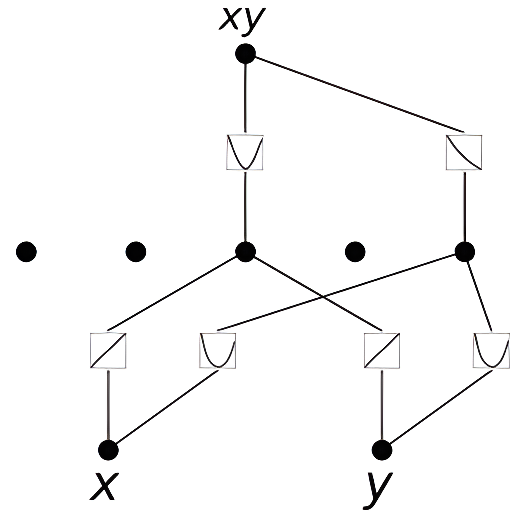
\includegraphics[width=5cm]{contents/images/pruning_example}
            \end{center}
        \end{column}

        \begin{column}{6cm}
            \begin{itemize}
                \item Function to be learned $f(x,y) = xy$ \vspace{1em}
                \item KAN computes: $$(x+y)^2 - (x^2+y^2)$$
                \item Note that: $$(x+y)^2 - (x^2+y^2) = 2xy$$
            \end{itemize}
        \end{column}
    \end{columns}
\end{frame}

\begin{frame}{Beating the COD (?)}
   \begin{itemize}
       \item The \textbf{curse of dimensionality (COD)} refers to the exponential growth in volume associated with adding more dimensions to a space \vspace{0.3em}
       \item UAT tells us that theoretically, a neural network with one hidden layer can approximate any function, but as the dimensionality of the input increases, the number of neurons required grows exponentially \vspace{0.3em}
       \item This leads to a MLP that is very large and potentially computationally intractable \vspace{0.3em}
       \item On the other hand, KAN's approximation ability is more dependent on the number of control points in each activation function and less on the data's dimension \vspace{0.3em}
       \item So, KAN's size will not increase exponentially as the data dimensions increase, but its grid should become more fine-grained \vspace{0.3em}
       \item However, we should note that the current implementation of KANs is not as optimized as the one for MLPs, so in practice the training times for high-dimensional data are comparable
   \end{itemize}
\end{frame}


\begin{frame}{Continual Learning}
   \begin{itemize}
       \item Catastrophic forgetting is a problem in MLPs \vspace{0.3em}
       \item When a MLPs is trained on one task and then  shifted to being trained on another, the network will soon forget about how to perform the first task \vspace{0.3em}
       \item Do you recall the motivation behind using splines to approximate curves instead of using polynomials? \strong{Locality!} \vspace{0.3em}
       \item Since spline bases are local, a sample will only affect a few nearby spline coefficients, leaving far-away coefficients intact \vspace{0.3em}
       \item This is desirable assuming faraway regions may have already stored information that we want to preserve \vspace{0.3em}
       \item By contrast, since MLPs usually use global activations any local change may propagate to regions far away \vspace{0.3em}
   \end{itemize}
\end{frame}